\documentclass[crop,tikz]{standalone}

\usepackage{pgfplots}
\tikzset{>=latex}

\pgfplotsset{
  inverted/.style = {
    every axis legend/.append style={
      draw=white,
      fill=hardblack,
      text=white
    }
  },
  every non boxed x axis/.append style={
    axis line style={-latex}
  },
  every non boxed y axis/.append style={
    axis line style={-latex}
  }
}

\begin{document}
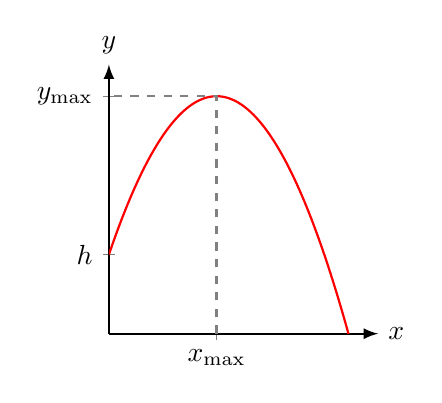
\begin{tikzpicture}
  \begin{axis}[
    height=5cm,
    width=5cm,
    thick,
    axis x line=middle,
    axis y line=middle,
    xlabel={$x$},
    ylabel={$y$},
    xlabel style={right},
    ylabel style={above},
    xtick={1},
    xticklabels={$x_{\max}$},
    ytick={0.5, 1.5},
    yticklabels={$h$, $y_{\max}$},
    xmin=0, xmax=2.5,
    ymin=0, ymax=1.7,
    samples=100,
    declare function = { f(\x) = -(\x - 1)^2 + 1.5; },
    ]
    \addplot[red,domain=0:2.3] { f(x) };
    \draw[gray,dashed] (axis cs:1,0) -- (axis cs:1,{f(1)}) -- (axis cs:0,{f(1)});
  \end{axis}
\end{tikzpicture}
\end{document}
